\documentclass[10pt,a4paper]{report}
\usepackage[utf8]{inputenc}

%\usepackage{fontspec}
%\setmonofont{consolas}

\usepackage[margin=1in]{geometry}

\usepackage{amsmath}
\usepackage{amsfonts}
\usepackage{amssymb}

% Graphic stuff
\usepackage{graphicx}
\usepackage{pgf, tikz}
\usetikzlibrary{automata, arrows}
\pgfdeclarelayer{background} 
\pgfsetlayers{background,main}

\usepackage{minted}
\usepackage{enumitem}

\title{
 \includegraphics[width=0.3\linewidth]{unifilogo.png} \\ \vspace{1cm}
 \Huge Homeworks of Bayesian Inference\\ {\LARGE (B004652) \\ \vspace{1cm} Group 1}}
\author{\LARGE Giovanni Papini}
\date{\vspace{3cm} \raggedleft Last revision: \today}

% Set `week`s instead of `chapter`s
\renewcommand{\chaptername}{Week}

% Homework details
\newcommand{\hmwkClass}{Bayesian Inference (B004652)}
\newcommand{\hmwkAuthorName}{Giovanni Papini}

% Headers
\usepackage{fancyhdr}

\pagestyle{fancy}
\lhead{\hmwkAuthorName}
\chead{\hmwkClass}
\rhead{\chaptername \space \thechapter}

% Probability commands: Expectation, Variance, Covariance, Bias
\DeclareMathOperator{\prob}{\mathbb P}
\DeclareMathOperator{\E}{E}
\DeclareMathOperator{\V}{V}
\DeclareMathOperator{\Var}{Var}
\DeclareMathOperator{\Cov}{Cov}

\newcommand{\Beta}{\text B}
\newcommand{\parm}{\mathord{\color{black!33}\bullet}}%

% Useful commands
\DeclareMathOperator{\blanket}{bl} % Markov blanket
\DeclareMathOperator{\logit}{logit}
\DeclareMathOperator*{\argmax}{arg \; max \;}
\DeclareMathOperator*{\argmin}{arg \; min \;}

\DeclareMathOperator{\iid}{i.i.d.}

% Hide subsection numeration
\renewcommand{\thesubsection}{}

\begin{document}
\maketitle

\part{}
\chapter{Exchangeability and stochastic processes}

\section{Exercise 1}

\subsection{Data}
\begin{itemize}
  \item $ E_1, E_2, E_3, E_4, E_5 $, events of simple alternative, exchangeable
  \item $ P(E_2) = \omega_1 = \frac{1}{2} $
  \item $ P(E_3 \wedge E_5) = \omega_2 = \frac{1}{4} $
  \item $ \omega_5 = \frac{\omega^5_3}{\binom{5}{3}} =
          \frac{\omega^5_1}{\binom{5}{1}} = \frac{1}{30} $
\end{itemize}

\subsection{Questions}
Compute:
\begin{enumerate}
  \item $ P(E_2 \wedge E_3 \wedge E_4) = \omega_3 $
  \item $ P(E_1 \wedge E_2 \wedge E_3 \wedge E_4) = \omega_4 $
  \item $ P(E_1 \wedge E_2 \wedge \bar E_3 \wedge
          \bar E_4 \wedge \bar E_5) = \frac{\omega_2^5}{\binom{5}{2}} $
\end{enumerate}

\subsection{Solutions}
First we find $ \omega_1^5 $ and $ \omega_3^5 $:
\begin{align*}
  \omega_1^5 & = \frac{1}{30} \cdot \binom{5}{1} = \frac{1}{6} \\
  \omega_3^5 & = \frac{1}{30} \cdot \binom{5}{3} = \frac{1}{3}
\end{align*}
Knowing that \[ \omega_h = \frac{1}{\binom{n}{h}} \sum_{r = h}^{n} \omega_r^n \binom{r}{h} \]
we can write that
\begin{align*}
  \omega_1 & = \frac{\omega_1^5 \binom{1}{1} + \omega_2^5 \binom{2}{1} +
    \omega_3^5 \binom{3}{1} + \omega_4^5 \binom{4}{1} + \omega_5^5 \binom{5}{1}}{\binom{5}{1}} \\
           & = \frac{1}{6} \cdot \frac{1}{5} + \frac{2}{5} \omega_2^5 +
  \frac{1}{5} \cdot \frac{1}{3} \cdot 3 + \frac{1}{5} \cdot 4 \omega_4^5 + \frac{1}{30}        \\
           & = \frac{8}{30} + \frac{2}{5} \omega_2^5 + \frac{4}{5} \omega_4^5                  \\ \\
  \omega_2 & = \frac{\omega_2^5 \binom{2}{2} +
    \omega_3^5 \binom{3}{2} + \omega_4^5 \binom{4}{2} + \omega_5^5 \binom{5}{2}}{\binom{5}{2}} \\
           & = \frac{1}{10} \omega_2^5 + \frac{1}{10} \cdot \frac{1}{10} \cdot 3 +
  \frac{1}{10} \cdot 6 \omega_4^5 + \frac{1}{30}                                               \\
           & = \frac{2}{15} + \frac{1}{10} \omega_2^5 + \frac{3}{5} \omega_4^5
\end{align*}
Combining them:
\begin{align*}
           & \begin{cases}
    \frac{2}{5} \omega_2^5 + \frac{4}{5} \omega_4^5 = \frac{1}{2} - \frac{8}{30} \\
    \frac{1}{10} \omega_2^5 + \frac{3}{5} \omega_4^5 = \frac{1}{4} - \frac{2}{15}
  \end{cases} \\
  \implies & \begin{cases}
    \omega_2^5 = \frac{7}{24} \\
    \omega_4^5 = \frac{7}{48}
  \end{cases}
\end{align*}
Now we can obtain
\begin{align*}
  \omega_3 & = \frac{\omega_3^5 \binom{3}{3} + \omega_4^5 \binom{4}{3} +
    \omega_5^5 \binom{5}{3}}{\binom{5}{3}}
           & = \frac{1}{3} \cdot \frac{1}{10} + \frac{7}{48} \cdot 4 \frac{1}{10} +
  \frac{1}{30} = \frac{1}{8}                                                          \\
  \omega_4 & = \frac{\omega_4^5 \binom{4}{4} + \omega_5^5 \binom{5}{4}}{\binom{5}{4}}
           & = \frac{7}{48} \cdot \frac{1}{5} + \frac{1}{30} = \frac{1}{16}
\end{align*}

\section{Exercise 2}

\subsection{Data}
\begin{itemize}
  \item Process of simple alternative $ \{| E_n |\} $
  \item $ P(E_1) = \omega_1 = \frac{1}{2} $
  \item $ P(E_1 \wedge E_2) = \omega_2 = \frac{1}{4} $
  \item $ P(E_1 \wedge E_2 \wedge E_3) = \omega_3 = \frac{1}{7} $
  \item $ P(E_1 \wedge E_2 \wedge E_3 \wedge E_4) = \frac{3}{28} $
\end{itemize}

\subsection{Questions}
\begin{enumerate}
  \item Could the 4 indicators $ |E_1| $, $ |E_2| $, $ |E_3| $ and $ |E_4| $ be
        the starting path of an exchangeable process?
  \item Could it continue for at least one step?
\end{enumerate}

\subsection{Solutions}
\begin{enumerate}
  \item An exchangeable process must satisfy the condition
        \[ (-1)^{n-h} \Delta^{n-h} \omega_h \ge 0,\; \forall n, h \le n \]
        Thus we compute
        \begin{itemize}
          \item $ (-1)^{4-1} \Delta^{4-1} \omega_1 =
                  (-1) \cdot \Delta^3 \omega_1 = \frac{1}{14} \ge 0 $
          \item $ (-1)^{4-2} \Delta^{4-2} \omega_2 =
                  (\phantom{-}1) \cdot \Delta^{2} \omega_2 = \frac{1}{14} \ge 0 $
          \item $ (-1)^{4-3} \Delta^{4-3} \omega_3 =
                  (-1) \cdot \Delta \; \omega_3 = \frac{1}{28} \ge 0 $
          \item $ (-1)^{4-4} \Delta^{4-4} \omega_4 =
                  (\phantom{-}1) \cdot \phantom{\Delta \;} \omega_4 = \frac{3}{28} \ge 0 $
        \end{itemize}
        Thus we can affirm that the process is exchangeable.
  \item If we consider $ n = 5 $ we can rewrite
        \begin{align*}
          - & \Delta\phantom{1} \omega_4 = \omega_4 - \omega_5 \ge 0 \implies
          \omega_5 \le \omega_4                                                                             \\
            & \Delta^2 \omega_3 = \omega_3 - 2 \omega_4 + \omega_5 \ge 0 \implies
          \omega_5 \ge 2 \omega_4 - \omega_3                                                                \\
          - & \Delta^3 \omega_2 = \omega_2 - 3 \omega_3 + 3 \omega_4 - \omega_5 \ge 0 \implies
          \omega_5 \le 3 \omega_4 - 3 \omega_3 + \omega_2                                                   \\
            & \Delta^4 \omega_1 = \omega_1 - 4 \omega_2 + 6 \omega_3 - 4 \omega_4 + \omega_5 \ge 0 \implies
          \omega_5 \ge 4 \omega_4 - 6 \omega_3 + 4 \omega_2 - \omega_1
        \end{align*}
        And substituting $ \omega_k $ with their values we obtain a system:
        \[
          \begin{cases}
            \omega_5 \le \frac{3}{28} \\
            \omega_5 \ge \frac{2}{28} \\
            \omega_5 \le \frac{3}{28} \\
            \omega_5 \ge \frac{2}{28}
          \end{cases} \implies
          \frac{2}{28} \le \omega_5 \le \frac{3}{28}
        \]
        Thus we can affirm that the process could continue.
\end{enumerate}

\chapter{Conjugate priors and posterior distributions}

\section{Exercise 2.3}

\subsection{Data}
\begin{itemize}
 \item $ p(x, y, z) \propto f(x, z) \; g(y, z) \; h(z) $
\end{itemize}

\subsection{Questions}
Prove that:
\begin{enumerate}
 \item $ p(x | y, z) \propto f(x, z) $
 \item $ p(y | x, z) \propto g(y, z) $
 \item $ X $ and $ Y $ conditionally independent, given $ Z $.
\end{enumerate}

\subsection{Solutions}
We know by definition that
\[ p(x | y, z) = \dfrac{p(x, y, z)}{p(y, z)} \]
and also that
\[
 p(y, z) = \int\limits_{S_X} p(x, y, z) \partial x \propto
 \int\limits_{S_X} f(x, z) g(y, z) h(z) \partial x =
 g(y, z) h(z) \int\limits_{S_X} f(x, z) \partial x
\]
Where $ S_X $ is the support of the r.v. $ X $. Then we can write
\begin{align*}
 p(x | y, z) & = \frac{f(x, z) g(y, z) h(z)}{g(y, z) h(z) \int_{S_X} f(x, z) \partial x} \\
             & = \frac{f(x, z)}{\int_{S_X} f(x, z) \partial x}
\end{align*}
But $ \int_{S_X} f(x, z) \partial x $ is constant given $ z $, so we can say
\[ p(x | y, z) \propto f(x, z) \]
as we wanted to show. \\
Similarly, we can write
\begin{align*}
 p(y | x, z) & = \frac{p(x, y, z)}{p(x, z)}                                              \\
             & = \frac{f(x, z) g(y, z) h(z)}{f(x, z) h(z) \int_{S_Y} g(y, z) \partial y} \\
             & = \frac{g(y, z)}{\int_{S_Y} g(y, z) \partial y}                           \\
             & \propto g(y, z)
\end{align*}
To show that $ X \perp Y $ given $ Z $ we have to prove that $ p(y | z, x) = p(y | z) $, so:
\begin{align*}
 p(y|z) & = \frac{p(y, z)}{p(z)}                              \\
        & = \frac{\int_{S_X} f(x, z) g(y, z) h(z) \partial x}
 {\int_{S_X}\int_{S_Y} f(x, z) g(y, z) h(z) \partial y \partial x} \\
        & = \frac{g(y, z) h(z)\int_{S_X} f(x, z) \partial x}
 {h(z) \int_{S_X} f(x, z) \partial x \int_{S_Y} g(y, z) \partial y} \\
        & = \frac{g(y, z)}{\int_{S_Y} g(y, z) \partial y}     \\
        & = p(y | x, z)
\end{align*}

\section{Exercise 3.5}

\subsection{Data}
\begin{itemize}
 \item $ p(y | \phi) = c(\phi) h(y) \exp(\phi t(y)) $
 \item $ p_1(\theta) \ldots p_k(\theta) $ conjugate priors
 \item $ \tilde{p}(\theta) = \sum_{k = 1}^{K} \omega_k p_k(\theta) $ where
       $ \omega_k > 0 $ and $ \sum_k \omega_k = 1 $
\end{itemize}

\subsection{Questions}
\begin{enumerate}
 \item $ p(\theta | y) $ as a function of $ p(y | \theta) $ and $ \tilde{p} $
 \item Previous question but in the case that $ \theta \sim \text{Pois} $ and
       $ p_1 \ldots p_k \sim \Gamma $
\end{enumerate}

\subsection{Solution}
For the Bayes rule:
\begin{align*}
 p(\theta | y) & = \frac{p(y | \theta) \cdot p(\theta)}{p(y)}                                            \\
               & = \frac{p(y | \theta) \cdot \tilde{p}(\theta)}{p(y)}                                    \\
               & = \frac{\prod_i p(y_i | \theta) \tilde{p}(\theta)}{p(y)}                                \\
               & = \frac{\prod_i c(\theta) h(y_i) \exp(\theta t(y_i)) \cdot \tilde{p}(\theta)}{p(y)}     \\
               & = \frac{\prod_i h(y_i) c(\phi)^n \exp(\phi \sum_i t(y_i)) \cdot \sum_k w_k p_k(\theta)}
 {\int_{S_\theta} \prod_i h(y_i) c(\phi)^n \exp(\phi \sum_i t(y_i)) \sum_k w_k p_k(\theta) \partial \theta} \\
               & = \frac{c(\phi)^n \exp(\phi \sum_i t(y_i)) \cdot \sum_k w_k p_k(\theta)}
 {\int_{S_\theta} c(\phi)^n \exp(\phi \sum_i t(y_i)) \sum_k w_k p_k(\theta) \partial \theta}
\end{align*}
In the particular case that $ p(y | \theta) $ is a Poisson distribution and $ p_k $ are Gamma
distribution, we have that
\begin{itemize}
 \item $ t(y) = y $
 \item $ \phi = \log(\theta) $
 \item $ c(\phi) = \exp(e ^ {-\phi}) = \exp(\theta^{-1}) $
 \item $ p_k(\theta) = \frac{\beta_k ^ {\alpha_k}}{\Gamma(\alpha_k)}
       \theta ^ {\alpha_k - 1} \exp(-\beta_k \theta) =
       c_k \theta ^ {\alpha_k - 1} \exp(-\beta_k \theta) $
\end{itemize}
So we can rewrite the posterior of the first part as
\begin{align*}
 p(\theta | y) & = \frac{\exp(\theta^{-1})^n \exp(\log \theta \sum_i y_i) \sum_k w_k c_k \theta^{\alpha_k - 1} \exp(-\beta_k \theta) }
 {\int_{S_\theta} \exp(\theta^{-1})^n \exp(\log \theta \sum_i y_i) \sum_k w_k c_k \theta^{\alpha_k - 1} \exp(-\beta_k \theta) \partial \theta} \\
               & = \frac{\exp(\theta^{-n}) \theta^{\sum_i y_i} \sum_k w_k c_k \theta ^ {\alpha_k - 1} \exp(-\beta_k \theta)}
 {\int_{S_\theta} \exp(\theta^{-n}) \theta^{\sum_i y_i} \sum_k w_k c_k \theta ^ {\alpha_k - 1} \exp(-\beta_k \theta) \partial \theta} \\
               & = \frac{\exp(\theta ^ {-n}) \sum_k w_k c_k \theta ^ {\alpha_k + \sum_i y_i - 1} \exp(-\beta_k \theta)}{} % TODO
\end{align*}

\chapter{Non informative priors}

\section{Exercise 3.10}

\subsection{Data}
\begin{itemize}
 \item $ \psi = g(\theta) $ where $ g $ is a monotone function
 \item $ h(\cdot) = g^{-1}(\cdot) $, that is $ \theta = h(\psi) $
 \item $ p_\theta(\theta) = \text{pdf of } \theta \implies
       p_\psi(\psi) = p_\theta(h(\psi)) \cdot \left|\frac{dh}{d\psi}\right|$
\end{itemize}

\subsection{Questions}
\begin{enumerate}
 \item Let $ \theta \sim Beta(a, b) $ and $ \psi = \logit(\theta) $. Obtain $ p_\psi $ and
       plot it for the case $ a = b = 1 $.
 \item Let $ \theta \sim Gamma(a, b) $ and $ \psi = \log(\theta) $. Obtain $ p_\psi $ and
       plot it for the case $ a = b = 1 $.
\end{enumerate}

\subsection{Solutions}
\begin{enumerate}
 \item The inverse function of $ \logit(\cdot) $ is known to be
       $ h(\psi) = \frac{\exp(\psi)}{1 + \exp(x\psi)} $, and the derivative w.r.t. $\psi$ of
       $ h(\psi) $ is
       \begin{align*}
        \frac{\partial h(\psi)}{\psi} & = \frac{\exp(\psi)(1 + \exp(\psi) - \exp(2\psi)}{(1 + \exp(\psi))^2} \\
                                      & = \frac{\exp(\psi)}{(1 + \exp(\psi))^2}
       \end{align*}
       So we can write the pdf of $\psi$ as
       \begin{align*}
        p_\psi(\psi) & = \frac{1}{B(a, b)} \left(\frac{\exp(\psi)}{1 + \exp(\psi)}\right)^{a - 1}
        \left(1 - \frac{\exp(\psi)}{1 + \exp(\psi)}\right)^{b - 1}
        \frac{\exp(\psi)}{(1 + \exp(\psi))^2} \\
                     & = \frac{1}{B(a, b)} \frac{\exp(\psi)^{a - 1}}{(1 - \exp(\psi))^{a - 1}}
        \frac{1}{(1 + \exp(\psi))^{b - 1}}
        \frac{\exp(\psi)}{(1 + \exp(\psi))^2} \\
                     & = \frac{1}{B(a, b)} \frac{\exp(\psi)^{a}}{(1 + \exp(\psi))^{a + b}}
       \end{align*}
       And in the case that $ a = b = 1 $ the plot is: \\
       \includegraphics[width=\textwidth]{julia-scripts/week-03_plot1.png}
       % Note: it seems very similar to a Normal distribution.
 \item The inverse function of $ \log(\theta) $ is known to be $ h(\psi) = \exp(\psi) $,
       and the derivative w.r.t. $\psi$ of $ h(\psi) $ is
       \[ \frac{\partial h(\psi)}{\partial \psi} = \exp(\psi) \]
       So we can write the pdf of $ \psi $ as
       \begin{align*}
        p_\psi(\psi) & = \frac{b ^ a}{\Gamma(a)} \exp(\psi)^{a - 1} \exp(-b\exp(\psi)) \exp(\psi) \\
                     & = \frac{b ^ a}{\Gamma(a)} \exp(a\psi - b\exp(\psi))
       \end{align*}
       And in the case that $ a = b = 1 $ the plot is: \\
       \includegraphics[width=\textwidth]{julia-scripts/week-03_plot2.png}
\end{enumerate}

\section{Exercise 3.14}

\subsection{Data}

\subsection{Questions}
\begin{enumerate}
 \item Given $ Y_1 \ldots Y_n \sim \text{Bernoulli}(\theta) $ find the MLE of $\theta$ and
       $ \frac{J(\theta)}{n} $.
 \item Find a pdf $ p_U(\theta) $ such that $ \log p_U(\theta) = l(\theta | \mathbf{y}) / n + c $
       where $ c $ is a constant that does not depend on $\theta$. Compute $ -\partial^2 \log p_U(\theta) / \partial^2 \theta $.
 \item Obtain a pdf for $\theta$ that is proportional to $ p_U(\theta) p(\mathbf{y} | \theta) $.
       Can this be considered a posterior for $ \theta $?
 \item Repeat previous points with $ Y_1 \ldots Y_n \sim \text{Poisson}(\theta) $.
\end{enumerate}

\subsection{Solutions}
\begin{enumerate}
 \item \begin{align*}
       \hat{\theta}_{MLE} & = \argmin_\theta l(\theta | \mathbf{y}) \\
       & = \argmin_\theta \log (\prod_i \theta ^ {y_i} (1 - \theta)^{1 - y_i}) \\
       & = \argmin_\theta \sum_i \log (\theta ^ {y_i} (1 - \theta) ^ {1 - y_i}) \\
       & = \argmin_\theta \log(\theta) \sum_i y_i + \log(1 - \theta) \sum_i (1 - y_i) \\
       & = \argmin_\theta \log(\theta) \sum_i y_i + n \log(1 - \theta) - \log(1 - \theta) \sum_i (y_i)
 \end{align*}
 To find the minimum we compute the zeros of $ \partial l(\theta | \mathbf{y}) / \partial \theta $
 \begin{align*}
  0 & = \frac{\partial l(\theta | \mathbf{y})}{\partial \theta}                                   \\
    & = \frac{\sum_i y_i}{\theta} - \frac{n}{1 - \theta} + \frac{\sum_i y_i}{1 - \theta}          \\
    & = \frac{\sum_i y_i - \theta \sum_i y_i - \theta n + \theta \sum_i y_i}{\theta (1 - \theta)} \\
    & = \frac{\sum_i y_i - \theta n}{\theta (1 - \theta)}
 \end{align*}
 Thus, if $ \theta \notin \left\{0, 1\right\} $, $ \hat \theta_{MLE} = \frac{\sum_i y_i}{n} $.
 \begin{align*}
  - \frac{\partial^2 l(\theta | \mathbf{y})}{n \partial^2 \theta}
    & = - \frac{-n \theta (1 - \theta) - (\sum_i y_i - n \theta)(1 - 2\theta)}{n \theta^2 (1 - \theta)^2} \\
    & = - \frac{n \theta^2 - n \theta - \sum_i y_i + 2\theta \sum_i y_i + n \theta - 2 n \theta^2}
  {n \theta^2 (1 - \theta^2)} \\
    & = \frac{n \theta ^ 2 - 2 \theta \sum_i y_i + \sum_i y_i}{n \theta^2 (1 - \theta)^2} \\
    & = \frac{\theta ^ 2 - 2 \theta \hat \theta_{MLE} + \hat \theta_{MLE}}{\theta^2 (1 - \theta)^2}
 \end{align*}
 The constrains on $ p_U(\theta) $ imply that 
 \[ p_U(\theta) = c \sqrt[n]{\prod_i \theta ^ y_i (1 - \theta) ^ {1 - y_i}} \]
 where $ c $ is the normalization constant.
\end{enumerate}

\chapter{Monte Carlo simulations}

\section{Exercise 1}

\subsection{Data}

\begin{itemize}
 \item Data sequence: \\
       \texttt{c(1, 1, 0, 0, 0, 0, 0, 1, 1, 1, 1, 1, 0, 0, 0, 0, 0, 0, 0, 0)}
\end{itemize}

\subsection{Questions}

Check that the sequence comes from an exchangeable process using the Bayesian
p-value and the number of switch as statistic test.

\subsection{Solutions}

Solution: $ 0.016 $ \\
Code:
\begin{minted}[fontsize=\footnotesize]{R}
set.seed(10)

count_switch <- function(x) x %>% diff() %>% abs() %>% sum()

y <- c(1, 1, 0, 0, 0, 0, 0, 1, 1, 1, 1, 1, 0, 0, 0, 0, 0, 0, 0, 0)
t_obs <- sum(abs(diff(y)))

# posterior hyperparameters
alpha <- 0.5 + sum(y)
beta  <- 0.5 + length(y) - sum(y)

niter <- 10000
ssize <- 20

theta <- rbeta(niter, alpha, beta)
t_rep <- map_dbl(theta, ~ rbinom(ssize, 1, .) %>% count_switch())

# Result
pval <- mean(t_rep <= t_obs)
cat("Bayesian p-val:", pval)
\end{minted}

\section{Exercise 2}

\subsection{Questions}

We want a sample from a distribution $ f(x) $ using another distribution $ g(x)
$ through an AR algorithm. Being assumed the value of $ M $, proof that this
algorithm is equivalent to a \textit{standard} AR.
\begin{enumerate}[label=\alph*)]
 \item Generate $ x \sim \text{G} $ \label{AR:step1}
 \item Generate $ u \sim \text{U}(0, M g(x)) $ \label{AR:step2}
 \item Accept $ y \overset{def}{=} x $ if $ u < f(x) $ \label{AR:step3}
 \item Otherwise go back to \ref{AR:step1}.
\end{enumerate}

\subsection{Solutions}

We can see that the two algorithms differ only for steps \ref{AR:step2} and
\ref{AR:step3}, where the difference is the Uniform distribution from which we
sample $ u $. To verify that they are equivalent we have to see if:
\begin{enumerate}
 \item The proportion of values accepted near a generic $ x $ is the same, that
       is equal to $ \frac{f(x)}{M g(x)} $, \label{AR:cond1}
 \item The efficiency is the same: the mean number of replications before
       rejecting a point is the same and it's equal to $ M $. \label{AR:cond2}
\end{enumerate}
In a generic $ u $ in the support of $ \text{U}(0, M g(x)) $ the proportion of
values below $ u $ is
\[ \prob(U < u) = \frac{u}{M g(x)} \]
therefor if $ u \overset{def}{=} f(x) $ the proportion of accepted values given
$ x $ is $ \frac{f(x)}{M g(x)} $, so \ref{AR:cond1} is verified.

Let $ K $ be the number of replications before accepting a value. So
\[ K \sim \text{Geom}(p) \text{ with $ p $ probability of accepting at each replication} \]
We can compute the expected value of acceptance probability:
\[ p = \prob(U \le f(x)) = \int_{S_X} g(x) \int_{0}^{f(x)} \frac{1}{M g(x)} \partial u \partial x = 
   \int_{S_X} g(x) \frac{f(x)}{M g(x)} \partial x = \frac{1}{M} \int_{S_X} f(x) \partial x = \frac{1}{M} \]
So the expected value $ \E[K] = \frac{1}{p} = M $ and even \ref{AR:cond2} is
verified, and we can affirm that the two procedures are equivalent.
\chapter{Unit information prior (again)}

\section{Exercise 5.5, Hoff}

\subsection{Questions}
\begin{enumerate}
  \item Reparametrize the normal model as $ p(y | \theta, \psi) $ where
        $ \psi = 1 / \sigma^2 $. Write the log-likelihood in terms of
        $\theta$ and $\psi$.
  \item Find a probability density $ p_U(\theta, \psi) $ so that $ \log(\theta, \psi) =
          l(\theta, \psi | \vect y) / n + c $ where $ c $ is a constant and does not
        depend on $\theta$ and $\psi$.
  \item Find a PDF $ p_U(\theta, \psi | \vect y) $, proportional to
        $ p_U(\theta, \psi) \cdot p(\vect y | \theta, \psi) $. Can this joint density considered
        a posterior PDF?
\end{enumerate}

\subsection{Solutions}
\begin{enumerate}
  \item \begin{align*}
          p(y | \theta, \psi) & = \frac{\sqrt{\psi}}{\sqrt{2\pi}} \exp\left( -\frac{\psi}{2} (y - \theta)^2 \right)
          \cdot \left| \frac{\partial \psi^{-\frac{1}{2}}}{\partial \psi} \right|                                          \\
                              & = \frac{3}{2} \psi^{-\frac{3}{2}} \frac{\sqrt{\psi}}{\sqrt{2\pi}}
          \exp\left( -\frac{\psi}{2} (y - \theta) ^2 \right)                                                               \\
                              & = \frac{3}{2} \frac{1}{\psi \sqrt{2\pi}} \exp\left( -\frac{\psi}{2} (y - \theta)^2 \right)
        \end{align*}
        \begin{align*}
          l(\theta, \psi | \vect y)
           & = \sum_{i = 1}^{n} \log\left\{ \frac{3}{2} \left( \frac{\psi}{\sqrt{2\pi}} \right)
          \exp \left(\frac{\psi(y_i - \theta)^2}{2} \right) \right\}                                          \\
           & = n \log\left( \frac{\psi}{\sqrt{2\pi}} \right) + \frac{\psi}{2} \sum_{i=1}^n (y_i - \theta)^2   \\
           & = n \log\left( \frac{\psi}{\sqrt{2\pi}} \right) + \frac{\psi}{2} \sum_{i=1}^n (y_i - \bar y)^2 +
          \frac{\psi}{2} \sum_{i=1}^n (\bar y - \theta)^2
        \end{align*}
  \item \begin{align*}
          l_U(\theta, \psi)
           & = \frac{l(\theta, \psi | \vect y)}{n} + c                                                                        \\
           & = \frac{1}{n} \left[ n \log\left( \frac{\psi}{2\pi} \right) - \frac{\psi}{2} \sum_i (y_i - \theta)^2 \right] + c \\
           & = \log\left( \frac{\psi}{\sqrt{2\pi}} \right) -
          \frac{\psi}{2n} \sum_i (y_i - \bar y)^2 - \frac{\psi}{2} (\bar y - \theta)^2 + c                                    \\
          \implies p_U(\theta, \psi)
           & \propto \exp( l_U(\theta, \psi) )                                                                                \\
           & \propto
          \underbrace{ \psi^2 \cdot \exp\left( -\frac{\sum_i (y_i - \bar y)^2}{2n} \cdot \psi \right) }_
          {\text{kernel of a Gamma($ 2 $, $ \sum_i (y_i - \bar y)^2 / 2n $)}}
          \underbrace{ \psi^{-1} \exp\left( -\frac{\psi}{2} (\theta - \bar y)^2 \right) }_
          {\text{kernel of a Normal($\bar y$, $\psi$)}}
        \end{align*}
  \item \begin{align*}
          p_U(\theta, \psi | \vect y)
           & \propto p_U(\theta, \psi) \cdot p(\vect y | \theta, \psi)                                      \\
           & \propto \psi^{-1} \exp\left( -\frac{\sum_i (y_i - \bar y)^2}{2n} \psi \right)
          \exp\left( -\frac{\psi}{2} (\theta - \bar y)^2 \right) \cdot
          \psi^{n} \exp\left( -\frac{\psi}{2} \sum_i (y_i - \theta)^2 \right)                               \\
           & \propto \psi^{n - 1}  \exp\left( -\frac{\sum_i (y_i - \bar y)^2}{2n} \psi \right)
          \exp\left( -\frac{\psi}{2} (\theta - \bar y)^2 -\frac{\psi}{2}\sum_i (y_i - \theta)^2 \right)     \\
           & = \psi^{n - 1}  \exp\left( -\frac{\sum_i (y_i - \bar y)^2}{2n} \psi \right) \cdot
          \exp\left( -\frac{\psi}{2} (\theta - \bar y)^2 - \frac{\psi}{2} \sum_i (y_i - \bar y)^2
          - \frac{\psi}{2} \sum_i (\bar y - \theta)^2 \right)                                               \\
           & \propto \underbrace{ \psi^{n}  \exp\left( -\frac{\sum_i (y_i - \bar y)^2 }{2n} \psi \right) }_
          { \text{kernel of a Gamma} } \cdot
          \underbrace{ \psi^{-1} \exp\left( -\frac{(n + 1) \psi}{2} (\theta - \bar y)^2 \right) }_
          { \text{kernel of a Normal} }
        \end{align*}
\end{enumerate}
\chapter{Gibbs sampler}

\section{Exercise 6.1, Hoff}

\subsection{Data}

\begin{itemize}
 \item Let's reconsider the number of children data in Exercise 4.8.
 \item Assume Poisson sampling models for the two groups as before, but
       parameterize $ \theta_A $ and $ \theta_B $ as $ \theta_A = \theta $
       and $ \theta_B = \theta_\gamma $, where $ \gamma $ is the relative
       rate $ \theta_B / \theta_A $. Let $ \theta \sim \text{Gamma}
       (a_\theta, b_\theta) $ and $ \gamma \sim \text{Gamma}(a_\gamma, b_\gamma) $.
\end{itemize}

\subsection{Questions}

\begin{enumerate}
 \item Are $ \theta_A $ and $ \theta_B $ independent or dependent under this
       prior distribution? In which situations is such a joint prior distribution
       justified?
 \item Obtain the form of the full conditional distribution of $ \theta $ given
       $ \mathbf y_A $, $ \mathbf y_B $ and $ \gamma $.
 \item Obtain the form of the full conditional distribution of $ \gamma $ given
       $ \mathbf y_A $, $ \mathbf y_B $ and $ \theta $.
 \item Set $ a_\theta = 2 $ and $ b_\theta = 1 $. Let $ a_\gamma = b_\gamma 
       \in \left\{8, 16, 32, 64, 128\right\} $. For each of these five values,
       run a Gibbs sampler of at least 5,000 iterations and obtain 
       $ \E[\theta_B - \theta_A | \mathbf y_A, \mathbf y_B] $. Describe the effects
       of the prior distribution for $ \gamma $ on the results.
\end{enumerate}

\subsection{Solutions}

\begin{enumerate}
 \item We evaluate the covariance expression of $ \theta_A $ and $ \theta_B $:
       \begin{align*}
        \Cov[\theta_A, \theta_B] 
          &= \E[\theta_A \theta_B] - \E[\theta_A] \E[\theta_B] \\
          &= \E[\theta ^ 2 \gamma] - \E[\theta] \E[\theta \gamma] \\
          &= \E[\theta ^ 2] \E[\gamma] - \E[\theta] ^ 2 \E[\gamma] \tag*{(for the independence of $ \theta $ and $ \gamma $)} \\
          &= \E[\gamma] (\E[\theta ^ 2] - \E[\theta] ^ 2) \\
          &= \E[\gamma] \Var[\theta] = \frac{a_\gamma}{b_\gamma} \frac{a_\theta}{b_\theta^2} > 0
       \end{align*}
      Thus the two variables are not independent.
      
      This kind of prior joint distribution could be useful in situations where 
      we are modeling the number of events in two different contests $ A $ and 
      $ B $ in a certain time interval and the mean number of events is respectively
      $ \theta_A $ and $ \theta_B $. The parameter $ \gamma $ can be interpreted as
      an acceleration factor caused by a phenomenon that change in the contest 
      $ B $, but that remains constant in the ``rest of the world'' $ A $.
      In this way of thinking $ \theta $ represents the \textit{standard} and 
      $ \gamma $ represents the element that, ceteris paribus, deviates from it.
      So, this parameterization of the prior joint is justified when we want to
      measure the intensity of the change caused to a starting population $ A $.
      As a consequence it lends itself well in experimental rather than observational 
      scopes.
\item First of all we observe the DAG that represents the relational model of variables.
      \begin{figure}[H]
       \centering
       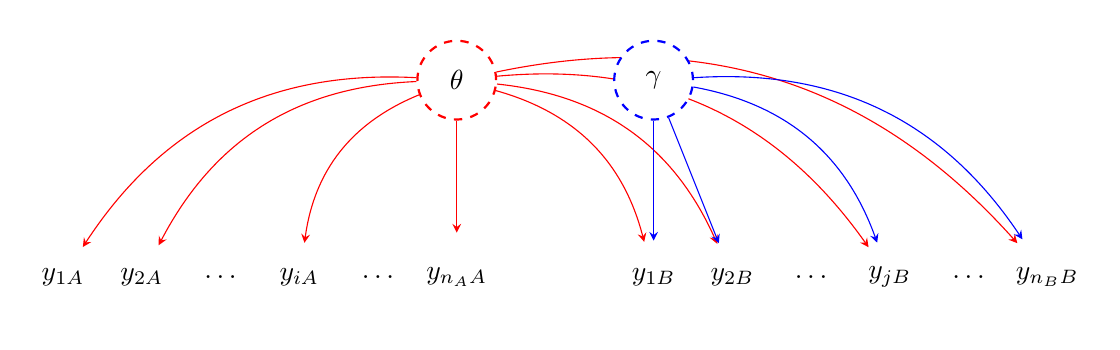
\begin{tikzpicture}[node distance=1cm]
        % styles %
        \tikzstyle{param} = [circle,thick,fill=white,dashed,minimum size=1cm];
        \tikzstyle{yobs} = [circle];
        \tikzstyle{thetadep} = [->, draw=red, fill=red, >=stealth];
        \tikzstyle{gammadep} = [->, draw=blue, fill=blue, >=stealth];
        
        % nodes %
        \node [param,draw=red] (theta) {$\theta$};
        \node [param,draw=blue] (gamma) [right of = theta, xshift = 1.5cm] {$\gamma$};
        
        \node [yobs] (ynA) [below of = theta, yshift=-1.5cm] {$ y_{n_AA} $};
        \node [yobs] (dt1) [left of = ynA] {$ \ldots $};
        \node [yobs] (yiA) [left of = dt1] {$ y_{iA} $};
        \node [yobs] (dt2) [left of = yiA] {$ \ldots $};
        \node [yobs] (y2A) [left of = dt2] {$ y_{2A} $};
        \node [yobs] (y1A) [left of = y2A] {$ y_{1A} $};
        
        \node [yobs] (y1B) [below of = gamma, yshift=-1.5cm] {$ y_{1B} $};
        \node [yobs] (y2B) [right of = y1B] {$ y_{2B} $};
        \node [yobs] (dt3) [right of = y2B] {$ \ldots $};
        \node [yobs] (yjB) [right of = dt3] {$ y_{jB} $};
        \node [yobs] (dt4) [right of = yjB] {$ \ldots $};
        \node [yobs] (ynB) [right of = dt4] {$ y_{n_BB} $};
        
        % edges %
        \begin{pgfonlayer}{background}
        \path[thetadep] (theta) 
                      edge node {} (ynA)
                      edge [bend right] node {} (yiA)
                      edge [bend right] node {} (y2A)
                      edge [bend right] node {} (y1A)
                      edge [bend left]  node {} (y1B)
                      edge [bend left]  node {} (y2B)
                      edge [bend left]  node {} (yjB)
                      edge [bend left]  node {} (ynB);
        \path[gammadep] (gamma)
                      edge node {} (y1B)
                      edge node {} (y2B)
                      edge [bend left] node {} (yjB)
                      edge [bend left] node {} (ynB);
        \end{pgfonlayer}
       \end{tikzpicture}
      \end{figure}
      
      \textbf{Full conditional of $\theta$} \quad The \textit{Markov blanket} of
      $\theta$ is 
      \[ \blanket(\theta) = \left\{ Y_{1A}, Y_{2A}, 
        \ldots, Y_{n_AA}, Y_{1B}, \ldots, Y_{n_BB}, \gamma \right\} \]
      in fact the $\theta$ node does not have parents and its children are all
      the observations. Moreover, for the $ B $ sample, $\gamma$ is another
      parent.
      \begin{align*}
       p(\theta\, |\, \blanket(\theta))
        &\propto p(\theta | a_\theta, b_\theta)\, \prod_{i = 1}^{n_A} p(Y_{iA} | \theta) 
         \prod_{j = 1}^{n_B} p(Y_{jB} | \theta, \gamma) \\
        &= \frac{b_\theta ^ {a_\theta}}{\Gamma(a_\theta)} \theta ^ {a_\theta - 1} \exp(-b_\theta \theta)
         \prod_{i = 1}^{n_A} \theta^{y_{iA}} \frac{\exp(-\theta)}{y_{iA}!}
         \prod_{j = 1}^{n_B} (\theta \cdot \gamma)^{y_{jB}} \frac{\exp(-\theta \gamma)}{y_{jB}!} \\
        &\propto \theta ^ {a_\theta - 1} \exp(-b_\theta \theta)
         \theta ^ {\sum_i y_{iA}} \exp(-n_A \theta) 
         (\theta \cdot \gamma) ^ {\sum_j y_{jB}} \exp(-n_B \theta) \\
        &= \theta ^ {a_\theta + \sum_i y_{iA} + \sum_j y_{jB} - 1} \exp(-(b_\theta + n_A + n_B)\theta)
      \end{align*}
      We can note the kernel of a Gamma distribution, so
      \[ \theta\, |\, \blanket(\theta) \sim \text{Gamma}(a_\theta + 
       \textstyle \sum_i y_{iA} + \textstyle \sum_j y_{jB},\, b_\theta + n_A + n_B) \]
\item \textbf{Full conditional of $\gamma$} \quad The \textit{Markov blanket} of 
      this random variable is
      \[ \blanket(\gamma) = \left\{ Y_{1B}, Y_{2B}, \ldots, Y_{n_BB}, \theta \right\} \]
      \begin{align*}
       p(\gamma\, |\, \blanket(\gamma))
        &\propto p(\gamma | a_\gamma, b_\gamma) \prod_{j = 1}^{n_B} p(y_{jB} | \theta, \gamma) \\
        &= \frac{b_\gamma ^ {a_\gamma}}{\Gamma(a_\gamma)} \gamma^{a_\gamma - 1} \exp(-b_\gamma \gamma)
         \prod_{j = 1}^{n_B} (\theta \cdot \gamma) ^ {y_{iB}} \frac{\exp(-\theta \gamma)}{y_{jB}!} \\
        &\propto \gamma ^ {a_\gamma - 1} \exp(-b_\gamma \gamma) 
         (\theta \cdot \gamma) ^ {\sum_j y_{jB}} \exp(-n_B (\theta \cdot \gamma)) \\
        &\propto \gamma ^ {a_\gamma + \sum_j y_{jB} - 1} \exp(-(b_\gamma + n_B\theta)\gamma)
      \end{align*}
      We can note the kernel of a Gamma distribution, so
      \[ \gamma\, |\, \blanket(\gamma) \sim \text{Gamma}(a_\gamma + \textstyle \sum_j y_{jB},\, 
       b_\gamma + n_B\theta) \]
\item At this point we can proceed with a simulation through the Gibbs algorithm following the MCMC
      approach.
\begin{minted}[fontsize=\small]{r}
library(tidyverse)

# Load data
yobs <- list(
    A = scan("data/menchild30bach.dat"),
    B = scan("data/menchild30nobach.dat")
)

# Hyperparameters
a_theta <- 2
b_theta <- 1
gammapriors <- 2 ^ (3:7)

# Sample statistics
ytot <- map(yobs, sum)
n <- map(yobs, length)

# Simulation main function
library(compiler) # to accelerate
gibbs_sim <- function(a_gamma, b_gamma = a_gamma, 
                      theta0 = 1, gamma0 = 1, nsim = 5000, seed = 10) {
    set.seed(seed)
    # Initialize
    result <- matrix(NA, nsim, 2, dimnames = list(NULL, c("theta", "gamma")))
    result[1, ] <- c(theta0, gamma0)
    # Main loop
    for (r in 2:nsim) {
        result[r, "theta"] <- rgamma(1, a_theta + ytot$A + ytot$B, 
                                     b_theta + n$A + n$B * result[r - 1, "gamma"])
        result[r, "gamma"] <- rgamma(1, a_gamma + ytot$B, b_gamma + n$B * result[r, "theta"])
    }
    # Return
    return(as_tibble(result))
}

# Simulation
simulations <- map(gammapriors, gibbs_sim, nsim = 1E4)
statistics <- map_dbl(simulations, ~ with(., mean(theta * gamma - theta)))
# [1] 0.3720311 0.3344181 0.2713526 0.2000735 0.1327382
\end{minted}
      We have evidence of the fact that the two means converge when the parameters
      of the prior distribution get higher. This imply that the difference gets lower
      and that the mean number of children in the two groups tends to be the same when
      we take higher hyper-parameters.
      
      We can see it even graphically comparing the posterior distributions of $ \theta_A $
      and $ \theta_B $ in the 5 configurations:
\begin{figure}[H]
 \centering
 \includegraphics[width=\linewidth]{r-scripts/week-06_hist.pdf}
\end{figure}
Code:
\begin{minted}[fontsize=\small]{R}
opar <- par(mfrow = n2mfrow(6))

for (j in seq_along(gammapriors)) {
    theta <- pluck(simulations, j, "theta")
    gamma <- pluck(simulations, j, "gamma")
    hist(theta, prob = TRUE, col = "lightblue", ylim = c(0, 5), xlim = c(0, 2.5),
         ylab = "posterior density", xlab = "mean number of children",
         main = substitute(paste(a[gamma], " = ", b[gamma], " = " , prior),
    list(prior = gammapriors[j])))
    lines(density(theta), col = "blue")
    hist(gamma * theta, prob = TRUE, col = "orange", add = TRUE)
    lines(density(gamma * theta), col = "red")
    legend("topleft", c(expression(theta[A]), expression(theta[B])),
           col = c("blue", "red"), lty = 1, cex = 0.7)
}

par(opar)
\end{minted}
      It's apparent even graphically that when the hyper-parameters of $\gamma$ increase, the
      posterior distributions get nearer, going even to overlap.
      
      This is due to the fact that the higher we sat the priors of $\gamma$, the more we
      weight the information that we already have about the variable, and consequently
      the observed information gain less importance.
      
      It's interesting even to observe how the Gamma distribution change when we set the
      different $ a_\gamma $ and $ b_\gamma $.
\begin{figure}[H]
 \centering
 \includegraphics[width=0.65\linewidth]{r-scripts/week-06_prior.pdf}
\end{figure}
      Code:
\begin{minted}[fontsize=\small]{r}
plot(NULL, xlim = c(0, 3), ylim = c(0, 4.5),
     xlab = expression(gamma), ylab = expression(p(gamma)),
     main = "Gamma prior")
for (i in seq_along(gammapriors)) {
    curve(dgamma(x, gammapriors[i], gammapriors[i]), add = TRUE, col = i)
}
legend_txt <- parse(text = paste("a[gamma] ==", gammapriors))
legend(x = 1.5, y = 3, legend_txt, col = seq_along(gammapriors), lty = 1)
mtext(expression(b[gamma] == a[gamma]))
\end{minted}
      As we can see the in the plot, the higher the hyper parameters we set, the
      more the distribution shrinks to 1, that is also the expected value of the
      Gamma. Vice versa, the variance decreases proportionally.
      
      Going toward the limit case in which $ a_\gamma $ and $ b_\gamma $ go to
      infinity we are implicitly affirming that we do not want to \textit{learn}
      anything from the new observations, and we already have a strong opinion
      about the Gamma that we don't want to change. However, if are talking from
      a Bayesian perspective, this situation is not sane neither useful; it's
      just a way to see how much the inference can change on the base of the
      choice of a priori distribution of parameters.
      
      \textbf{Observation} \quad It would be appropriate to adequately assess
      the convergence of the Gibbs algorithm, but in this case it was not done
      because it was not explicitly requested by the exercise. We just calculate
      the effective sample size and make sure it is high enough to make sure we
      have reached the equilibrium distribution and have it very close to it.
      
\begin{minted}[fontsize=\small]{r}
library(coda)
map(simulations, effectiveSize)

# [[1]]
# theta    gamma
# 1175.254 1198.183
#
# [[2]]
# theta    gamma
# 1471.870 1353.061
#
# [[3]]
# theta    gamma
# 1840.738 1695.119
#
# [[4]]
# theta    gamma
# 2424.931 2238.538
#
# [[5]]
# theta    gamma
# 3259.088 2942.661
\end{minted}
\end{enumerate}

\part{}
\chapter{Hierarchical models, part 1}

\section{Exercise 8.1, Hoff}

\subsection{Data}
\begin{itemize}
 \item Consider the hierarchical model where
       \begin{align*}
        \theta_1, \ldots, \theta_m   | \mu, \tau^2        & \sim \iid \Normal(\mu,
        \tau^2)
        \\
        y_{1, j}, \ldots, y_{n_j, j} | \theta_j, \sigma^2 & \sim \iid \Normal(\theta_j,
        \sigma^2)
       \end{align*}
\end{itemize}

\subsection{Questions}
\begin{enumerate}[label=\alph*)]
 \item Which do you think is bigger, $ \Var[y_{i, j} | \theta_i, \sigma^2] $ or $
        \Var[y_{i, j} | \mu, \tau^2] $?
 \item Do you think $ \Cov[y_{i_1, j}, y_{i_2, j} | \theta_j, \sigma^2] $ is negative,
       positive or zero?
       Answer the same for $ \Cov[y_{i_1, j}, y_{i_2, j} | \mu, \tau^2] $.
 \item Compute the quantities and compare with the intuitive results.
 \item Assuming that we had a prior $ p(\mu) $ for $\mu$. Using the Bayes' rule, show
       that
       \[ p(\mu | \theta_1, \ldots, \theta_m, \tau^2, \sigma^2, \vect y_1, \ldots, \vect
        y_m) =
        p(\mu | \theta_1, \ldots, \theta_m, \tau^2) \]
       Interpret in words what this means.
\end{enumerate}

\subsection{Solutions}
\begin{enumerate}[label=\alph*)]
 \item $ \Var[y_{i, j} | \mu, \tau^2] $ will be intuitively the higher one, because we
       are \textit{constraining}
       fewer variables.
 \item The two variables $ y_{i_1, j} $ and $ y_{i_2, j} $ will be independent given $
        \theta_j $, for definition.
       Yet, if I condition only on $ \mu $ and $ \tau^2 $, the two variables will have a
       positive covariance; in fact
       if I observe a high value of $ y_{i_1, j} $ I expect to see a similar value for $
        y_{i_2, j} $ and vice versa.
 \item \begin{align*}
        \intertext{\raggedleft By definition, we know that $ y_{i, j} | \theta_j,
          \sigma^2
          \sim \Normal(\theta_j, \sigma^2) $}
        \Var[y_{i, j} | \theta_j, \sigma^2]
         & = \sigma^2
        \\
        \intertext{\raggedleft We can apply the property of variance of independent
         variables,
         \\
         because $ y_{i, j} | \theta_j, \sigma^2 $ are i.i.d.}
        \Var[\bar y_j | \theta_j, \sigma^2]
         & = \Var\left[ \frac{1}{n} \sum_{i = 1}^{n} y_{i, j} | \theta_j, \sigma^2
         \right]
        \\
         & = \frac{1}{n} \sum_{i = 1}^{n} \Var[y_{i, j} | \theta_j, \sigma^2] =
        \frac{\sigma^2}{n_j}
        \\
        \intertext{\raggedleft Again using the property that $ y_{i, j} $ are i.i.d.,
         given
         $ \theta_j $ and $ \sigma^2 $}
        \Cov[y_{i_1, j}, y_{i_2, j} | \theta_j, \sigma^2]
         & = 0
        \\
        \intertext{\centering The first intuition of point b) was correct, and justified
         by theory.}
       \end{align*}

       \setlength{\fboxsep}{10pt} % increase the spacing of fbox
       \fbox{\parbox{\textwidth}{ % put everything inside a frame
         \textbf{Note} \quad This quantities concern variables conditioned to a generic
         group \textit{j},
         and it is straightforward to obtain them even in a frequentist point of view.
         The next variances require to consider these theorems of probability theory:
         \begin{enumerate}
          \item \textbf{Law of total variance}: \\
                Given two random variables $ X $ and $ Y $ with $ \Var[X] < \infty $,
                then:
                \begin{equation}\label{week7:eq_totalvariance}
                 \Var[X] = \E[\Var[X | Y]] + \Var[\E[X | Y]]
                \end{equation}
          \item \textbf{Law of total covariance}: \\
                Given three random variables $ X $, $ Y $ and $ Z $ with $ \Cov[X, Y] <
                 \infty $, then:
                \begin{equation}\label{week7:eq_totalcovariance}
                 \Cov[X, Y | Z] = \E[\Cov[X, Y | Z]] + \Cov[\E[X | Z] \cdot \E[Y | Z]]
                \end{equation}
         \end{enumerate}
        }}

       \begin{align*}
        \intertext{\raggedleft Thus, we can apply here \ref{week7:eq_totalvariance} with
         $ X = y_{i, j} $ and $ Y = \theta_j $}
        \Var[y_{i, j} | \mu, \tau^2]
         & = \E[\Var[y_{i, j} | \theta_j, \mu, \tau^2]] + \Var[\E[y_{i, j} | \theta_j,
          \mu,
          \tau^2]]
        \\
         & = \E[\Var[y_{i, j} | \theta_j, \sigma^2, \mu, \tau^2]] +
        \Var[\E[y_{i, j} | \theta_j, \sigma^2, \mu, \tau^2]]
        \\
         & = \E[\sigma^2] + \Var[\theta_j | \mu, \tau^2]
        \\
         & = \sigma^2 + \tau^2 > \sigma^2
        \\
        \intertext{\centering The intuition at point a) is confirmed.}
        \intertext{\raggedleft We apply again \ref{week7:eq_totalvariance}, with $ X =
          \bar y_j $ and $ Y = \theta_j $}
        \Var[\bar y_j | \mu, \tau^2]
         & = \E[\Var[\bar y_j | \theta_j, \mu, \tau^2]] + \Var[\E[\bar y_j | \theta_j,
          \mu,
          \tau^2]]
        \\
         & = \E[\Var[\bar y_j | \theta_j, \sigma^2, \mu, \tau^2]] +
        \Var[\E[\bar y_j | \theta_j, \sigma^2, \mu, \tau^2]]
        \\
         & = \E[\frac{\sigma^2}{n_j}] + \Var[\theta_j | \mu, \tau^2] =
        \frac{\sigma^2}{n_j}
        + \tau^2
        \\
        \intertext{\raggedleft Lastly, we use \ref{week7:eq_totalcovariance} for the last
         term with
         $ X = y_{i_1, j} $, $ Y = y_{i_2, j} $ and $ Z = \theta_j $}
        \Cov[y_{i_1, j}, y_{i_2, j} | \mu, \tau^2]
         & = \E[\Cov[y_{i_1, j}, y_{i_2, j} | \theta_j, \mu, \tau^2]]
        \\
         & + \Cov[\E[y_{i_1, j} | \theta_j, \mu, \tau^2] \cdot \E[y_{i_2, j} | \theta_j,
          \mu, \tau]]
        \\
         & = \E[0] + \Cov[\theta_j, \theta_j | \mu, \tau^2]
        \\
         & = 0 + \Var[\theta_j | \mu, \tau^2] = \tau^2 > 0
        \intertext{\centering Even the second intuition of the point b) was correct.}
       \end{align*}
       \textbf{Note} \quad Another analytic solution could be to calculate the marginal
       distribution of $ y_{i, j} | \mu, \tau^2 $ as
       \[ p(y_{i, j} | \theta_j, \mu, \tau^2) =
        \int_{\theta_j \in \Theta} p(y_{i, j} | \theta_j, \mu, \tau^2) \cdot p(\theta_j |
        \mu, \tau^2) \partial \theta_j \]
       Since both of them are normal distributions, we expect it to be another normal,
       and we have only to verify that
       the variance is equal to $ \Var[y_{i, j} | \mu, \tau^2] $ as previously computed.
       The same for the other quantities.
 \item First of all, we represent the hierarchical model through a DAG
       \begin{figure}[H]
        \centering
        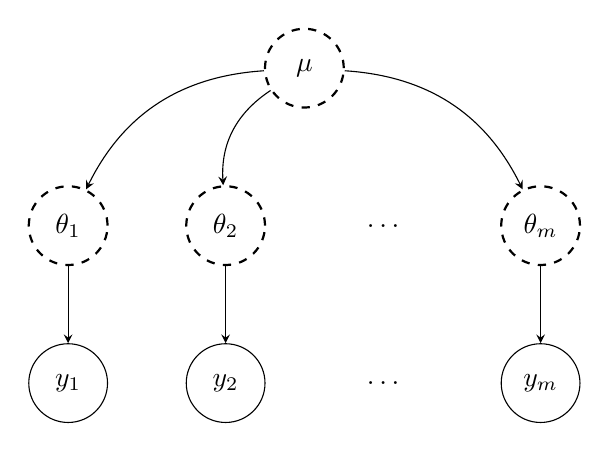
\begin{tikzpicture}[node distance=1cm,->,draw=black,>=stealth]
         % styles %
         \tikzstyle{param} = [circle,thick,draw=black,fill=white,dashed,minimum
         size=1cm];
         \tikzstyle{yobs} = [circle,draw=black,fill=white,minimum size=1cm];

         % nodes %
         \node [param] (mu) {$\mu$};

         \node [param,below of=mu, yshift=-1cm, xshift=-1cm] (theta2) {$\theta_2$};
         \node [param,draw=white,below of=mu, yshift=-1cm, xshift=1cm] (thetadots)
         {$\ldots$};
         \node [param,left of=theta2, xshift=-1cm] (theta1) {$\theta_1$};
         \node [param,right of=thetadots, xshift=1cm] (thetam) {$\theta_m$};

         \node [yobs,below of=theta1,yshift=-1cm] (y1) {$\vect y_1$};
         \node [yobs,below of=theta2,yshift=-1cm] (y2) {$\vect y_2$};
         \node [yobs,draw=white,below of=thetadots,yshift=-1cm] (ydots) {$\ldots$};
         \node [yobs,below of=thetam,yshift=-1cm] (ym) {$\vect y_m$};

         % edges %

         \path (mu)
         edge [bend right] node {} (theta1)
         edge [bend right] node {} (theta2)
         edge [bend left] node {} (thetam);
         \path (theta1) edge node {} (y1);
         \path (theta2) edge node {} (y2);
         \path (thetam) edge node {} (ym);
        \end{tikzpicture}
       \end{figure}
       Using this graph and its factorization one can calculate the conditioned
       probability as
       \begin{align*}
        p(\mu | \theta_1, \ldots, \theta_m, \tau^2, \sigma^2, \vect y_1, \ldots, \vect
        y_m)
         & = \frac{p(\mu, \theta_1, \ldots, \theta_m, \tau^2, \sigma^2, \vect y_1,
         \ldots,
         \vect y_m)}
        {p(\theta_1, \ldots, \theta_m, \tau^2, \sigma^2, \vect y_1, \ldots,
         \vect y_m)}
        \\
         & = \frac{p(\mu, \theta_1, \ldots, \theta_m, \tau^2, \sigma^2, \vect y_1,
         \ldots,
         \vect y_m)}
        {\int p(\mu, \theta_1, \ldots, \theta_m, \tau^2, \sigma^2, \vect y_1,
         \ldots, \vect y_m) \dd \mu}
        \\
         & = \frac{p(\vect y_1, \ldots, \vect y_m | \theta_1, \ldots, \theta_m, \sigma^2)
         \cdot
         p(\theta_1, \ldots, \theta_m | \mu, \tau^2) \cdot p(\mu)}
        {\int p(\vect y_1, \ldots, \vect y_m | \theta_1, \ldots, \theta_m,
         \sigma^2) \cdot
         p(\theta_1, \ldots, \theta_m | \mu, \tau^2) \cdot p(\mu) \dd \mu}
        \\
         & = \frac{p(\vect y_1, \ldots, \vect y_m | \theta_1, \ldots, \theta_m, \sigma^2)
         \cdot
         p(\theta_1, \ldots, \theta_m | \mu, \tau^2) \cdot p(\mu)}
        {p(\vect y_1, \ldots, \vect y_m | \theta_1, \ldots, \theta_m, \sigma^2)
         \cdot
         \int p(\theta_1, \ldots, \theta_m | \mu, \tau^2) \cdot p(\mu) \dd \mu}
        \\
         & = \frac{p(\theta_1, \ldots, \theta_m | \mu, \tau^2) \cdot p(\mu)}
        {\int p(\theta_1, \ldots, \theta_m | \mu, \tau^2) \cdot p(\mu) \dd \mu}
        \\
         & = \frac{p(\theta_1, \ldots, \theta_m, \mu, \tau^2)}{p(\theta_1, \ldots,
         \theta_m, \tau^2)}
        \\
         & = p(\mu | \theta_1, \ldots, \theta_m, \tau^2) \tag*{$ \square $}
       \end{align*}

       This result implies that the information obtained from the samples in a
       certain sense does not refer \textit{directly} on the grand mean, but it
       passes trough the inference that we do on $\theta$s. In fact, the grand mean
       is independent of the observations conditioned $ \theta_1, \ldots, \theta_m $.
\end{enumerate}

\section{Exercise on continuous mixture models}

\subsection{Data}
\begin{itemize}
 \item If $ y|\theta \sim \Poisson(\theta) $ and $ \theta \sim \Gammadist(\alpha,
       \beta) $, then the marginal (prior predictive) distribution of $ y $ is a
       negative binomial with parameters $\alpha$ and $\beta$ (or $ p = \beta / (1 +
       \beta) $).
 \item In the Normal model with unknown location and scale ($\mu$, $\sigma^2$),
       the non informative prior density, $ p(\mu, \sigma) \propto 1 / \sigma^2 $,
       results in a normal-inverse-$\chi^2$ posterior distribution. Marginally then
       $ \sqrt{n} (\mu - \bar y) / s $ has a posterior distribution $ t_{n - 1} $,
       where $ s^2 = \sum_i (y_i - \bar y)^2 / (n - 1) $ is the sample
       variance of the observation.
\end{itemize}

\subsection{Questions}
\begin{enumerate}[label=\alph*)]
 \item Derive the mean and the variance of the negative binomial.
 \item Derive the first two moments of the latter distribution, stating the
       appropriate condition on $n$ for existence of both of them.
\end{enumerate}

\subsection{Solutions}
\begin{enumerate}[label=\alph*)]
 \item We can leverage on the property of the expected value that, given two variables
       $ X $ and $ Y $
       \begin{equation}\label{week7:eq_condexpectation}
        \E_X[X] = \E_Y[\E_X[X | Y]]
       \end{equation}
       Thus,
       \begin{align*}
        \E_y[y] & = \E_\theta[\E_y[y | \theta]] \\
                & = \E_\theta[\theta]           \\
                & = \frac{\alpha}{\beta}
       \end{align*}

       For the variance, we can refer to \ref{week7:eq_totalvariance} and consider
       $ X = y $ and $ Y = \theta $
       \begin{align*}
        \Var[y] & = \E[\Var[y | \theta]] + \Var[\E[y | \theta]]   \\
                & = \E[\theta] + \Var[\theta]                     \\
                & = \frac{\alpha}{\beta} + \frac{\alpha}{\beta^2} \\
                & = \frac{(1 + \beta) \alpha}{\beta^2}
       \end{align*}

       \textbf{Formal alternative} \quad Using the following parameterization:
       \[ p(x | \theta, r) = \binom{x - 1}{r - 1} \theta ^{r} (1 - \theta) ^{x - r} \]
       with $ \theta = \beta / ( 1 + \beta) $ and $ r = \alpha $.

       \begin{align*}
        \E[x] & = \sum_{x \in \Theta} x \cdot p(x)
        \\
              & = \sum_{x = r}^{\infty} x \cdot \binom{x - 1}{r - 1} \cdot \theta ^r (1 -
        \theta) ^{x - r}
        \\
              & = \sum_{x = r}^{\infty} x \cdot \frac{(x - 1)!}{(r - 1)!(x - r)!} \cdot
        \theta ^r (1 - \theta) ^{x - r}
        \\
              & = r \cdot \sum_{x = r}^{\infty} \frac{x!}{r!(x - r)!} \cdot \theta ^r (1
        -
        \theta) ^{x - r}
        \intertext{\raggedleft Increment the lower index of the summation
         \\
         and decrement the index in the summand}
              & = \frac{r}{\theta} \cdot \sum_{x = r + 1}^{\infty} \binom{x - 1}{(r + 1)
         -
         1}
        \theta ^{r + 1} (1 - \theta) ^{x - (r + 1)}
        \intertext{\raggedleft The series is the sum of the PDF function of a $
          \text{NegBin}(\theta, r + 1) $
         \\
         all along its support, thus it is equal to 1}
              & = \frac{r}{\theta}
       \end{align*}

       To obtain the variance we recur to the equality
       \begin{equation}\label{week7:eq_variance}
        \Var[X] = \E[X^2] - \E[X]^2
       \end{equation}
       so, we obtain first of all $ \E[X^2] $.
       \begin{align*}
        \E[X^2]          & = \sum_{x = r}^{\infty} x^2 \cdot \binom{x - 1}{r - 1} \cdot
        \theta ^r
        (1 - \theta) ^{x - r}
        \\
                         & = \sum_{x = r}^{\infty} [x(x + 1) - x] \binom{x - 1}{r - 1}
        \cdot \theta
        ^r (1 - \theta) ^{x - r}
        \\
                         & = \sum_{x = r}^{\infty} [x(x + 1)] \binom{x - 1}{r - 1} \cdot
        \theta ^r
        (1 - \theta) ^{x - r} -
        \sum_{x = r}^{\infty} x \cdot \binom{x - 1}{r - 1} \cdot \theta ^r (1 -
        \theta) ^{x - r}
        \\
        \intertext{\raggedleft Following the same reasoning of the mean
         expression:
         \\
         multiply and divide for $ r $ and then $ r + 1 $}
                         & = \frac{r(r + 1)}{\theta ^2} \sum_{x = r + 2} \binom{x + 1}{r
         + 1} \theta
        ^{x + 2} (1 - \theta) ^{x - (r + 2)} -
        \frac{r}{\theta}
        \\
                         & = \frac{r(r + 1)}{\theta ^2} - \frac{r}{\theta}
        \\
                         & = \frac{r^2 + r - \theta r}{\theta ^2}
        \\
                         & = \frac{r^2}{\theta^2} + \frac{(1 - \theta) r}{\theta^2}
        \\
        \intertext{\raggedleft Now we can apply \ref{week7:eq_variance}}
        \implies \Var[X] & = \frac{r^2}{\theta^2} + \frac{(1 - \theta) r}{\theta^2} -
        \left( \frac{r}{\theta} \right)^2
        \\
                         & = \frac{(1 - \theta)r}{\theta ^ 2}
       \end{align*}
 \item The PDF of Student's t distribution
       \[ p(x | n) = c \cdot \left( 1 + \frac{x^2}{n} \right)^{-\frac{n + 1}{2}} \]
       where the c is a constant
       \[ c = \frac{1}{\sqrt{n}} \frac{1}{\Beta\left( \frac{n}{2}, \frac{1}{2}
       \right)} \]
       and $ \Beta(\parm, \parm) $ is the Beta function.

       It's immediate to see that the function is even, because $ x $ is present
       only as $ x^2 $, hence $ f(-x) = f(x) $.
       \begin{align*}
        \E[X] & = \int_{x \in \Theta} x \cdot f(x)  \dd x                         \\
              & = \int_{-\infty}^{\infty} x \cdot f(x) \dd x                      \\
              & = \int_{-\infty}^{0} x \cdot f(x) \dd x +
        \int_{0}^{\infty} x \cdot f(x) \dd x                                      \\
        \intertext{\raggedleft Change of variable in the first
         integral                                                                 \\$ t =
         -x $}
              & = -\int_{\infty}^{0} (-t) \cdot f(-t) \dd t +
        \int_{0}^{\infty} x \cdot f(x) \dd x                                      \\
              & = \phantom{-} \int_{\infty}^{0} \phantom{-} t \cdot f(-t) \dd t +
        \int_{0}^{\infty} x \cdot f(x) \dd x                                      \\
              & = -\int_{0}^{\infty} t \cdot f(-t) \dd t +
        \int_{0}^{\infty} x \cdot f(x) \dd x                                      \\
        \intertext{\raggedleft Since $ f(x) = f(-x) $}
              & = -\int_{0}^{\infty} t \cdot f(t) \dd t + \int_{0}^{\infty} x
        \cdot f(x) \dd x = 0
       \end{align*}
       The equality to 0 is granted by the finiteness of the two integrals, that
       is true only if the parameter $ n $ of the distribution is strictly
       greater then 1. In fact
       \begin{align*}
        \int_{0}^{\infty} x f(x) \dd x
         & = \lim\limits_{u \to \infty} \int_{0}^{u} x \cdot c \cdot
        \left( 1 + \frac{x^2}{n} \right)^{-\frac{1}{2}(n + 1)} \dd x    \\
         & = c \cdot \lim\limits_{u \to \infty} \left.
        -\frac{n}{n - 1} \left( 1 + \frac{x^2}{n} \right)^{-\frac{1}{2}(n - 1)}
        \right| _{0} ^{u}                                               \\
         & = -\frac{c \cdot n}{n - 1} \left( \lim\limits_{u \to \infty}
        \left( 1 + \frac{u^2}{n} \right)^{-\frac{1}{2}(n - 1)} - 1 \right)
       \end{align*}
       And the above limit is finite only if $ n > 1 $.

       \begin{align*}
        \E[X^2]
         & = \int_{x \in \Theta} x^2 \cdot f(x) \dd x
        \\
         & = \int_{-\infty}^{\infty} x^2 \cdot c \cdot \left( 1 + \frac{x^2}{n}
        \right)^{-\frac{n + 1}{2}} \dd x
        \intertext{\raggedleft Change of variable $ t = \left( 1 + \frac{x^2}{n}
          \right)^{-1} $}
         & = n ^{\frac{3}{2}} \cdot c \cdot \int_{0}^{1} t ^{\frac{n}{2} - 2} (1 - t)
        ^{\frac{1}{2}} \dd t
        \\
        \intertext{\raggedleft Note that the integrand function is the kernel of a Beta
         distribution,
         \\
         thus its result is known.}
         & = n ^{\frac{3}{2}} \cdot c \cdot \Beta\left( \frac{n}{2} - 1, \frac{3}{2}
        \right)
        \\
         & = n ^{\frac{3}{2}} \cdot \frac{1}{\sqrt{n} \Beta\left( \frac{n}{2},
         \frac{1}{2}
         \right)} \cdot
        \Beta\left( \frac{n}{2} - 1, \frac{3}{2} \right)
        \\
         & = n \cdot \frac{\Gamma\left( \frac{n}{2} + \frac{1}{2} \right)}
        {\Gamma\left( \frac{n}{2} \right) \Gamma\left( \frac{1}{2}
         \right)}
        \frac{\Gamma\left( \frac{n}{2} - 1 \right) \Gamma\left( \frac{3}{2}
         \right)}
        {\Gamma\left( \frac{n}{2} + \frac{1}{2} \right)}
        \\
        \intertext{\raggedleft By the property of the Gamma function that
         \\
         $ \Gamma(x) = (x - 1) \Gamma(x - 1) $}
         & = n \cdot \frac{\Gamma\left( \frac{n}{2} - 1 \right) \frac{1}{2} \Gamma\left(
         \frac{1}{2} \right)}
        {\left(\frac{n}{2} - 1\right) \Gamma\left( \frac{n}{2} - 1
         \right) \Gamma\left( \frac{1}{2} \right)}
        \\
         & = \frac{n}{n - 2}
       \end{align*}
       In this case the condition is $ n > 2 $, otherwise the integral of the
       Beta distribution does not converge.
\end{enumerate}

\end{document}
